\subsection{Growing samples and the blind spot}\label{sec:An}

\begin{figure}[t]
\centering
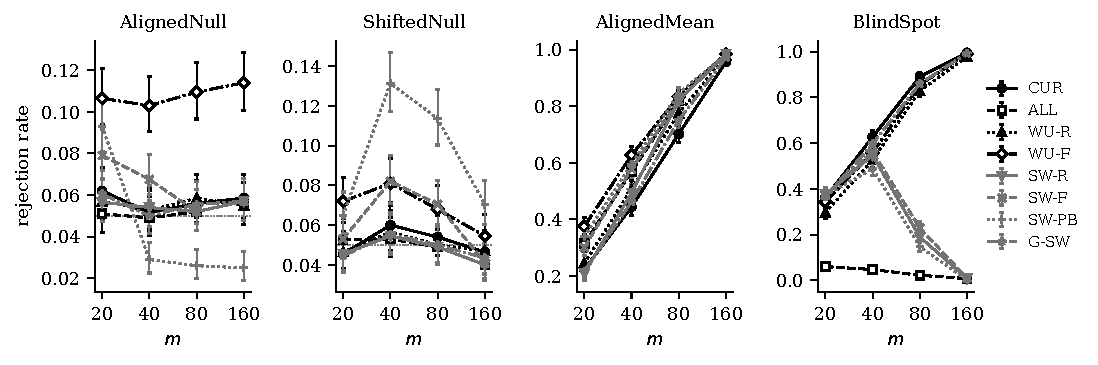
\includegraphics[width=\textwidth]{gen/fig_A_n.pdf}
\caption{A\_n: rejection rates against $m$ ($n=\ell_j=2m$, three sources, $\theta=0.5$) with Wilson 95\% intervals; dotted line at $0.05$ in null panels. BlindSpot: all sources $N(0.6,1)$ and $Q_t=\frac17N(0,1)+\frac67N(0.6,1)$, so pooling all sources reproduces $Q_t$. Full table in \cref{tab:An}.}\label{fig:An}
\end{figure}

\Cref{fig:An} and \cref{tab:An} show three patterns.

\paragraph{Frozen selection: which inflation vanishes.} SW-F rejected at $0.079$ at $m=20$ and $0.057$ at $m=160$ under AlignedNull, and at $0.082$ ($m=40$) and $0.041$ ($m=160$) under ShiftedNull. This matches the oracle-coupling mechanism: with a fixed radius and fixed distributions, the sourcewise selection stabilises (identical and $N(0.6,1)$ sources are eventually always accepted), and the conditioning effect fades. Frozen \emph{risk weights} (WU-F) stayed at $0.10$--$0.11$ under AlignedNull for every $m$. Soft weights never stabilise: $m\hat D^2/\hat v_c$ has a nondegenerate limit, so the selected weights remain random at every sample size. The original partial bootstrap (SW-PB) was anti-conservative at small $m$ ($0.093$, $0.132$) and, when merged sources are identical, conservative at larger $m$ ($0.025$--$0.029$). With shifted merged sources it stayed above $0.05$ up to $m=160$ ($0.070$).

\paragraph{Reselected and fixed-rule procedures stay calibrated.} Across the $8$ null cells, CUR, ALL, WU-R and SW-R stayed between $0.040$ and $0.062$. Two cells marked $\uparrow$ for CUR (an exact test) and one for G-SW are within the range expected from about $40$ marginal intervals. As a separate check, $20{,}000$ additional current-only tests with $m=20$ gave $0.0506$ (s.e.\ $0.0015$).

\paragraph{The blind spot is real and is removed by risk weighting.} In BlindSpot, ALL has power $0.060,0.047,0.022,0.007$ as $m$ grows, and SW-R, SW-F and SW-PB fall to $0.009$, $0.009$ and $0.001$ at $m=160$, while current-only testing reaches $0.994$. This is \cref{thm:blind} in action: for $m\ge80$ every source passes the fixed-radius fusion test, and the pooled control equals $Q_t$. WU-R follows the current-only curve from slightly below ($0.296$ vs.\ $0.361$ at $m=20$; $0.978$ vs.\ $0.994$ at $m=160$), as \cref{cor:uniform} predicts, and G-SW repairs SW-R ($0.992$). With aligned sources, SW-R gains up to $0.12$ ($m=80$: $0.820$ vs.\ $0.702$) and WU-R up to $0.07$.

\paragraph{Cost.} Per data set, SW-R took $0.10$, $0.16$, $0.20$ and $0.89$\,s at $m=20,40,80,160$ (row-wise fusion bootstrap), and WU-R took $0.09$--$0.17$\,s.

\subsection{Independent-seed confirmation}\label{sec:confirm}
\IfFileExists{sec_confirm_A.tex}{The complete A\_main design ($2000$/$1000$ replicates) and A\_n design ($1000$/$500$) were rerun with base seed $20261019$. \Cref{tab:confirm} compares the key quantities; the full confirmation null table is in \cref{app:additional} (\cref{tab:nullconf}).

\begin{table}[H]
\centering\scriptsize
\caption{Key quantities in the exploratory and the independent confirmation runs, with Wilson 95\% intervals (rates) or paired normal 95\% intervals (differences).}\label{tab:confirm}
\begin{tabular}{@{}lll@{}}
\toprule
Quantity & exploratory (seed 20261018) & confirmation (seed 20261019)\\
\midrule
max null rate over 5 scenarios, CUR & 0.059 [0.049, 0.070] & 0.051 [0.042, 0.061]\\
max null rate over 5 scenarios, WU-R & 0.057 [0.047, 0.067] & 0.054 [0.045, 0.065]\\
max null rate over 5 scenarios, SW-R & 0.054 [0.045, 0.065] & 0.057 [0.048, 0.068]\\
max null rate over 5 scenarios, G-WU & 0.053 [0.044, 0.064] & 0.050 [0.041, 0.060]\\
max null rate over 5 scenarios, WU-F & 0.126 [0.112, 0.141] & 0.123 [0.110, 0.139]\\
max null rate over 5 scenarios, SW-F & 0.096 [0.083, 0.109] & 0.097 [0.084, 0.110]\\
max null rate over 5 scenarios, SW-PB & 0.139 [0.125, 0.155] & 0.161 [0.145, 0.177]\\
WU-R $-$ CUR, Aligned, Mean$+$ & +0.063 [+0.045, +0.081] & +0.072 [+0.052, +0.092]\\
WU-R $-$ CUR, Aligned, Scale & +0.110 [+0.086, +0.134] & +0.119 [+0.095, +0.143]\\
WU-R $-$ CUR, Shifted, Mean$-$ & +0.103 [+0.084, +0.122] & +0.087 [+0.068, +0.106]\\
WU-R $-$ CUR, Shifted, Mean$+$ & -0.139 [-0.160, -0.118] & -0.124 [-0.145, -0.103]\\
WU-R $-$ CUR, Opposite, Scale & -0.148 [-0.171, -0.125] & -0.153 [-0.177, -0.129]\\
G-WU $-$ CUR, Shifted, Mean$+$ & -0.066 [-0.081, -0.051] & -0.056 [-0.071, -0.041]\\
WU-F null rate, AlignedNull, $m=160$ & 0.114 [0.101, 0.129] & 0.097 [0.080, 0.117]\\
SW-R power, BlindSpot, $m=160$ & 0.009 [0.005, 0.017] & 0.008 [0.003, 0.020]\\
WU-R power, BlindSpot, $m=160$ & 0.978 [0.967, 0.985] & 0.988 [0.974, 0.994]\\
CUR power, BlindSpot, $m=160$ & 0.994 [0.987, 0.997] & 0.994 [0.983, 0.998]\\
\bottomrule
\end{tabular}
\end{table}

Every qualitative conclusion is reproduced. Procedures with guaranteed level stayed at or below $0.057$ in the worst of five scenarios, frozen selections were again inflated ($0.123$, $0.097$ and $0.161$ for WU-F, SW-F and SW-PB), and the frozen risk weights remained inflated at $m=160$ ($0.097$). The power differences agree in sign and approximately in size: gains of $+0.07$ to $+0.12$ with compatible sources or opposing shifts, and losses of $-0.12$ to $-0.15$ when the source shift mimics the effect. The blind spot (SW-R power $0.008$ at $m=160$) and its removal by risk weighting ($0.988$) were also reproduced. Differences between the runs are within Monte Carlo error, except that the worst frozen partial-bootstrap rate is somewhat higher in the confirmation run ($0.161$ vs.\ $0.139$), which strengthens the conclusion.
}{Confirmation runs pending.}
